% Sketch output, version 0.3 (build 2d, Wed Apr 20 23:38:45 2011)
% Output language: PGF/TikZ,LaTeX
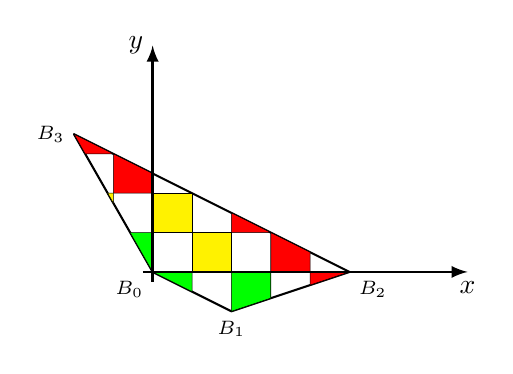
\begin{tikzpicture}[line join=round,line width=0.2pt,>=latex]
\filldraw[fill=none,line width=0.75pt](0,-4)--(1,-4.5)--(2.5,-4)--(-1,-2.25)--cycle;
\filldraw[fill=red](2,-4.167)--(2.5,-4)--(2,-4)--cycle;
\filldraw[fill=red](1.5,-4)--(2,-4)--(2,-3.75)--(1.5,-3.5)--cycle;
\filldraw[fill=red](1,-3.25)--(1,-3.5)--(1.5,-3.5)--cycle;
\filldraw[fill=red](-.5,-2.5)--(-.5,-3)--(0,-3)--(0,-2.75)--cycle;
\filldraw[fill=red](-1,-2.25)--(-.857,-2.5)--(-.5,-2.5)--cycle;
\filldraw[fill=yellow](.5,-4)--(1,-4)--(1,-3.5)--(.5,-3.5)--cycle;
\filldraw[fill=yellow](0,-3)--(0,-3.5)--(.5,-3.5)--(.5,-3)--cycle;
\filldraw[fill=yellow](-.5,-3)--(-.5,-3.125)--(-.571,-3)--cycle;
\filldraw[fill=green](1,-4.5)--(1.5,-4.333)--(1.5,-4)--(1,-4)--cycle;
\filldraw[fill=green](0,-4)--(.5,-4.25)--(.5,-4)--cycle;
\filldraw[fill=green](0,-4)--(0,-3.5)--(-.286,-3.5)--cycle;
\draw[->,line width=1pt](0,-4.125)--(0,-1.125);
\draw[->,line width=1pt](-.125,-4)--(4,-4);

    \coordinate [label=below:$x$] (X) at (4,-4);
    \coordinate [label=left:$y$] (Y) at (0,-1.125);
  
    \coordinate [label=225:\scriptsize$B_0$] (p0B) at (0,-4);
    \coordinate [label=270:\scriptsize$B_1$] (p1B) at (1,-4.5);
    \coordinate [label=-60:\scriptsize$B_2$] (p2B) at (2.5,-4);
    \coordinate [label=180:\scriptsize$B_3$] (p3B) at (-1,-2.25);
  \end{tikzpicture}% End sketch output
